\chapter{Теория} % Main chapter title

\label{Theory} % Change X to a consecutive number; for referencing this chapter elsewhere, use \ref{ChapterX}

\newcommand{\lrarr}{\Leftrightarrow}

%%%%%%%%%%%%%%%%%%%%%%%%%%%%%%%%%%%%%%%%%%%%%%%%%%%%%%%%%%%%%%%%%%%%%%%%%%%%%%%%%%%%%%%%%%%

В этой главе мы рассмотрим подходы для нахождения оптимального вектора вероятностей. Будут представлены аналоги greedy, $\epsilon$-greedy, стратегий с позитивной инициализацией, UCB, Gradient bandits, а также некоторые замечания по сэмплированию Томпсона.  

\section{Формализация задачи}

\subsection{Постановка задачи}

Итак, еще раз повторим задачу: имеется $n$ рычагов, $i$-ый рычаг соответствует какому-то распределению $\xi_i$ со средним $m_i$ и дисперсией $\sigma_i^2$. Распределения изначально неизвестны. Каждый ход мы можем выбрать один из рычагов, при выборе $i$-го рычага мы получаем награду, сгенерированную из $\xi_i$. После $t$-го шага у нас имеется вектор вероятностей $\tbf{p}_t = (p_1^t, ..., p_n^t)$, $\forall i \: p_i \geq 0$, и на $t+1$-ом шаге вероятность выбора $i$-го рычага равна $p_i^t$. Задача -- за $T$ шагов по получаемым наградам максимизировать $V = m_p - \lambda \cdot \sigma_p^2 = \sum_{i=1}^n p_i^T m_i - \lambda \sum_{i=1}^n (p_i^T)^2 \sigma_i^2$, где $\lambda > 0$. Максимизация достигается путем нахождения такого вектора вероятностей $\tbf{p}^*$, что $\tbf{p}^* = \underset{\tbf{p} \in \Delta^n}{\arg \max} \sum_{i=1}^n p_i m_i - \lambda \sum_{i=1}^n p_i^2 \sigma_i^2$. Далее всегда будем считать, что в первый ход рычаг выбирается случайно, то есть $\tbf{p}_1 = \left( \frac{1}{n}, ..., \frac{1}{n} \right)$. \\

В некоторых случаях у распределения нет дисперсии. Например, это верно для распределения Стьюдента $t_2$ с двумя степенями свободы. Если дисперсии нет у распределения $\zeta$, то считаем, что любое распределение $\xi_i \sim c_i \cdot \zeta$, и ставится задача максимизации $V = \sum_{i=1}^n p_i^T m_i - \lambda \sum_{i=1}^n (p_i^T)^2 c_i^2$, то есть в качестве меры риска берется ''растяжение'' $\xi_i$ относительного какого-то эталонного распределения $\zeta$.

\subsection{Обозначения}

Введем обозначения:
\begin{itemize}
    \item $R_t$ -- награда, полученная на $t$-ом шаге (то есть сразу после того момента, когда нажали на рычаг в $t$-ый раз).
    \item $A_t$ -- номер рычага, выбранный на $t$-ом шаге.
    \item $R_t(a) = R_t \cdot \bb{I}(A_t = a)$.
    \item $N_t(a) := \sum_{i=1}^{t-1} \bb{I}(A_t = a)$ -- количество нажатий на рычаг $a$ на $t$-ом шаге (перед процедурой нажатия в $t$-ый раз). Соответственно, на нулевом шаге $\forall a \hook N_t(a) = 0$.
    \item $Q_t(a) := \frac{\sum_{i=1}^{t-1} R_i(a)}{N_t(a)}$ -- средняя награда рычага $a$ на шаге $t$. Можно считать, что обновление происходит так: если на шаге $t$ было выбрано действие $a$, то для всех остальных действий $b$ значение $Q_t(b)$ не меняется, а для действия $a$ $Q_t(a) = Q_t(a) + \frac{1}{N_{t}(a) + 1}(R_t - Q_t(a))$. Заметим, что $Q_t(a)$ является выборочным матожиданием рычага $a$ по всем полученным от его нажаатия наградам.
    % \item $\bar{R_t} := \frac{\sum_{i=1}^{t-1} R_i}{max(t-1,1)}$ -- средняя награда за все предыдущие шаги, или, как ее называют по-другому, baseline.
    \item $\overline{R_t^2(a)} = \frac{\sum_{i=1}^{t-1} R_i^2(a)}{N_t(a)}$ -- средняя квадратичная награда рычага $a$ на шаге $t$. Аналогично средней награде, можно считать, что каждый ход происходит обновление только одного значения.
    \item $S_t^2(a) = \frac{1}{N_t(a) - 1}\sum_{i=1}^{t-1}(R_i(a) - Q_t(a))^2 = \frac{N_t(a)}{N_t(a) - 1}(\overline{R_t^2(a)} - Q_t(a)^2)$ -- выборочная дисперсия. Если $N_t(a) \leq 1$, будем считать, что $S_t^2(a) = 0$.
\end{itemize}

\subsection{Подсчет матожидания и дисперсии}

Будем приближать матожидание и дисперсию рычагов с помощью выборочного матожидания и выборочной дисперсии соответственно. Заметим, что $\bb{E} \, Q_t(a) = m_a$, $\bb{E} \, S_t(a) = \sigma_a^2$ (за исключением холодного старта, то есть случая $N_t(a) \leq 1$), и такие приближения корректны. Кроме того:
\begin{itemize}
    \item Для невыбранных на $t$-ом шаге рычагов обновления выборочного матожидания и дисперсии не происходит.
    \item $Q_{t+1}(A_t) = Q_t(A_t) + \frac{1}{N_{t}(A_t) + 1}(R_t - Q_t(A_t))$, поэтому обновление выборочного матожидания происходит за $O(1)$.
    \item $\overline{R_{t+1}^2(A_t)} = \overline{R_t^2(A_t)} + \frac{1}{N_{t}(A_t) + 1}(R_t^2 - \overline{R_t^2(A_t)})$ -- подсчет тоже происходит за $O(1)$.
    \item Так как $S_t^2(a) = \frac{N_t(a)}{N_t(a) - 1}(\overline{R_t^2(a)} - Q_t(a)^2)$, а $\overline{R_t^2(a)}$ и $Q_t(a)^2$ пересчитываются за $O(1)$, то и $S_t^2(a)$ пересчитывается за $O(1)$.
\end{itemize}

\section{Жадные стратегии}

В классической задаче о многоруких бандитах под жадной стратегией подразумевался выбор каждый ход рычага с наибольшим выборочным матожиданием, то есть $A_t = \underset{a}{\arg \max} Q_t(a)$. Поскольку это самая простая стратегия, она страдает от проблемы холодного старта: представим себе 2 рычага, $m_1 > m_2 > 0$. Пусть на первом шаге был прожат второй рычаг. Поскольку $m_2 > 0$, то велика вероятность получения награды $R_1 > 0$, так что $0 = Q_2(1) < Q_2(2) = R_1$. Поэтому далее снова прожмется второй рычаг и так далее. Поскольку по ЗБЧ $Q_t(2) \to m_2 > 0$, то с высокой вероятностью $\forall t \hook Q_t(2) > 0$ (особенно если $m_2$ сильно больше нуля), и первый рычаг никогда не выберется, хотя он дает большее матожидание. 

\subsection{Итеративные жадные стратегии}
\label{subsec:theory_iterative}

В отличие от обычной задачи о многоруких бандитах, в измененной версии для жадных стратегий вектор вероятностей выбора рычагов $\tbf{p}_t$ может быть не равен вектору $(0, ..., 1, 0, ..., 0)$. Каждый шаг будем менять вероятность выбора каждого рычага в соответствии с новой полученной наградой. ``Жадность'' будет выражаться в несколько другом смысле. Опишем сначала процесс изменения вероятностей для итеративных greedy-стратегий. Под итеративными стратегиями будем понимать стратегии, которые при заданных матожиданиях и дисперсиях сходятся к оптимальному вектору вероятностей за $k > 1$ проходов какого-то кода, но на каждом шаге производящих только один проход этого кода.

Пусть на $t$-ом шаге вектор вероятностей равен $\tbf{p}_t = (p_1^t,...,p_n^t)$. Будем на каждом шаге изменять вероятности так, чтобы максимально увеличить $V = Q_{t,p} - \lambda S_{t,p}^2$, где $Q_{t,p} = \sum_{i=1}^n p_i^t Q_t(i)$, $S_{t,p}^2 = \sum_{i=1}^n (p_i^t)^2 S_t(i)^2$. Можно рассмотреть 2 подхода.

\subsubsection{Изменение двух вероятностей}
\label{subsubsec:iterative_greedy_changing_two_probs}

Далее для облегчения обозначений будем вместо $p_t^i$ использовать $p_i$, а вместо $p_{t+1}^i$ -- $p_i^{new}$. \\ 
Каждый ход будем увеличивать одну из вероятностей $p_i$ на $\Delta p \geq 0$, а другую вероятность $p_j$ -- уменьшать на $\Delta p$. Сумма вероятностей не изменилась.Будем искать такие $i, \, j, \, \Delta p$, что $p_i^{new} \leq 1, p_j^{new} \geq 0$ и увеличение 
$V$ (обозначим за $\Delta V$) максимально. Заметим, что $p_i + \Delta p \leq 1 \lrarr \Delta p \leq 1 - p_i, \; p_j - \Delta p \geq 0 \lrarr \Delta p \leq p_j$ и $1 - p_j \geq p_i \lrarr p_i + p_j \leq 1$, поэтому условие $p_i^{new} \leq 1$ избыточно. После изменения соответствующих вероятностей получим:

\begin{equation}
\begin{split}
    \Delta V & = \Bigl[ (p_i + \Delta p) Q_t(i) + (p_j - \Delta p) Q_t(j) \\
             & - \lambda (p_i + \Delta p)^2 S_t^2(i) - \lambda (p_j - \Delta p) S_t^2(j) \Bigr] \\ 
             & - \left[  p_i Q_t(i) + p_j Q_t(j) - \lambda p_i^2 S_t^2(i) - \lambda p_j^2 S_t^2(j) \right] \\
             & = \Delta p (Q_t(i) - Q_t(j)) - 2 \lambda \Delta p (p_i S_t^2(i) - p_j S_t^2(j)) - \lambda (\Delta p)^2 \left[ S_t^2(i) + S_t^2(j) \right] \\ 
             & = \Delta p \left( [Q_t(i) - 2 \lambda p_i S_t^2(i)] - [Q_t(j) - 2 \lambda p_j S_t^2(j)]\right) - \lambda (\Delta p)^2 \left[ S_t^2(i) + S_t^2(j) \right] \\ 
             & \overset{w_k := Q_t(k) - 2 \lambda p_k S_t^2(k)}{=} (w_i - w_j) \Delta p - \lambda \left[ S_t^2(i) + S_t^2(j) \right] (\Delta p)^2
\end{split}
\end{equation}
Если $\lambda > 0$, $S_t^2(i) \neq 0 \lor S_t^2(j) \neq 0$, то получили квадратный многочлен с отрицательным главным коэффициентом. Этот многочлен достигает максимума в точке $\Delta p = \frac{w_i - w_j}{2 \lambda (S_t^2(i) + S_t^2(j))}$ и этот максимум равен $\frac{(w_i - w_j)^2}{4 \lambda \left[ S_t^2(i) + S_t^2(j) \right]}$. Заметим, что $w_i - w_j = - (w_j - w_i)$ и поэтому при перестановке $i$ и $j$ значение $\Delta p$ изменится на противоположное. Поэтому $p_i + \Delta p$ и $p_j - \Delta p$ не изменятся, как и ограничения на них. Для удобства будем рассматривать только такие пары $(i,j)$, что $w_i - w_j \geq 0$. Так как отрезок $\left[0, \min \left(p_j, \frac{w_i - w_j}{2 \lambda \left[ S_t^2(i) + S_t^2(j) \right]} \right) \right]$ находится левее точки максимума, то при заданных ограничениях максимум $\Delta V$ достигается при 
\[
\Delta p = \min \left( p_j, \frac{w_i - w_j}{2 \lambda \left[ S_t^2(i) + S_t^2(j) \right]} \right)
\]
Посчитав $\Delta V$ для всех пар $(i,j)$ с $w_i - w_j > 0$, сможем найти оптимальные $i, \, j, \, \Delta V$.

Если $S_t^2(i) = S_t^2(j) = 0$, то многочлен равен $\Delta p (Q_t(i) - Q_t(j)$. Опять, можно считать, что $Q_t(i) \geq Q_t(j)$, так как иначе знак $\Delta p$ меняется на противоположный, и максимальное значение $\Delta V$ не меняется. Тогда оптимальное $\Delta p = p_j$ и $\max \Delta V = (Q_t(i) - Q_t(j)) p_j$. Тот факт, что $S_t^2(i) = 0$, означает, что или количество нажатий на $i$-ый рычаг $ \leq 1$, или $i$-ый рычаг всегда выдаёт одно и то же значение (то есть рычаг безрисковый), или распределение $i$-го рычага дискретное, но все полученные до этого значения при нажатии на $i$-ый рычаг были одинаковыми. В случае, когда оба рычага безрисковые, и эти 2 рычага были выбраны для изменения вероятностей, $p_j^{new} = 0$, то есть безрисковый рычаг с меньшим значением больше не будет выбираться, как и в оптимальном векторе вероятностей. 

Обратим внимание на проблему холодного старта: после первого шага, когда был выбран только один $i$-ый рычаг, может оказаться, что полученная награда $> 0$, в то время как выборочные дисперсии всех рычагов и выборочное матожидание всех других рычагов нулевое. В таком случае наибольшая разница $\Delta V$ будет достигаться при увеличении вероятности выбранного рычага на $\frac{1}{n}$ и уменьшении вероятности какого-то другого рычага $j$ до $p_j^{new} = 0$. То есть $j$-ый рычаг больше не будет выбран, хотя он может быть ``лучше'' $i$-го рычага. Если же полученная награда $< 0$, то тогда обнулится вероятность выбора $i$-го рычага, хотя нам могло просто не повезти с наградой. О том, как справляться с этой проблемой, мы поговорим позднее.

Кроме того, алгоритм каждый шаг меняет всего 2 вероятности, что медленно, а сам шаг совершается за $O(n^2)$ (в то время как greedy-стратегия в обычной задаче о многоруких бандитах -- за $O(n)$).
    

\subsubsection{Изменение всех вероятностей}
\label{subsec:theory_iterative_change_all_probs}

В качестве альтернативы можно пытаться за один шаг менять сразу все вероятности. Одна из вероятностей будет изменяться в одну сторону, а остальные -- в другую. Отдельно будем рассматривать случаи с увеличением этой единственной вероятности и с ее уменьшением.
    
Пусть на $t$-ом шаге $\phi_t$ рычагов с ненулевыми вероятностями выбора, то есть $|\{i: p_t^i \neq 0\}| = \phi_t$ и пусть $K_t := \{i: p_t^i \neq 0\}$. Будем каждый ход увеличивать одну из вероятностей $p_i$ на $\Delta p_{\uparrow}$, а все остальные ненулевые вероятности -- уменьшать на $\frac{\Delta p_{\uparrow}}{\phi_{t,i}}$, где $\phi_{t,i} := \phi_t - \bb{I}_{p_i \neq 0}$. Сумма вероятностей не изменилась. Будем искать такие $i, \, \Delta p_{\uparrow}$, что $\forall j \hook 1 \geq p_j^{new} \geq 0$ и значение $\Delta V_{\uparrow}$ максимально. Если $\phi_{t,i} = 0$, то $p_i = 1$, и $\Delta p_{\uparrow} = \Delta V_{\uparrow} = 0$. Иначе после изменения соответствующих вероятностей получим:
\begin{dmath}
    \Delta V_{\uparrow} = \Delta p_{\uparrow} \left(Q_t(i) - \frac{\sum_{\substack{j \in K_t \\ j \neq i}} Q_t(j)}{\phi_{t,i}} \right) - 2\lambda \Delta p_{\uparrow} \left( p_i S_t^2(i) - \frac{\sum_{\substack{j \in K_t \\ j \neq i}} p_j S_t^2(j)}{\phi_{t,i}} \right) - \lambda (\Delta p_{\uparrow})^2 \left( S_t^2(i) + \frac{\sum_{\substack{j \in K_t \\ j \neq i}} S_t^2(j)}{\phi_{t,i}^2} \right) = \Delta p_{\uparrow} \left( w_i - \frac{\sum_{\substack{j \in K_t \\ j \neq i}} w_j}{\phi_{t,i}} \right) - \lambda (\Delta p_{\uparrow})^2 \left( S_t^2(i) + \frac{\sum_{\substack{j \in K_t \\ j \neq i}} S_t^2(j)}{\phi_{t,i}^2} \right) = \Delta p_{\uparrow} \frac{\sum_{\substack{j \in K_t \\ j \neq i}} (w_i - w_j)}{\phi_{t,i}} - \lambda (\Delta p_{\uparrow})^2 \frac{\sum_{\substack{j \in K_t \\ j \neq i}} (\phi_{t,i} S_t^2(i) + S_t^2(j))}{\phi_{t,i}^2}
    \label{eq:3}
\end{dmath}
Если $\lambda \neq 0$ и $\exists j \in K_t \cup \{i\} \hook S_t^2(j) \neq 0$, то получаем квадратный многочлен, максимум которого в точке
\[
\Delta p_{\uparrow} = \frac{\phi_{t,i} \sum_{\substack{j \in K_t \\ j \neq i}} (w_i - w_j)}{2\lambda \sum_{\substack{j \in K_t \\ j \neq i}} ( \phi_{t,i} S_t^2(i) + S_t^2(j) )}
\]
и в этой точке достигается значение
\[
\Delta V_{\uparrow} = \frac{\left( \sum_{\substack{j \in K_t \\ j \neq i}} (w_i - w_j) \right)^2}{4\lambda \sum_{\substack{j \in K_t \\ j \neq i}} ( \phi_{t,i} S_t^2(i) + S_t^2(j) )}
\]
Здесь уже может быть $\Delta p_{\uparrow} < 0$. Если $\Delta p_{\uparrow} \geq 0$, то налагаются дополнительные ограничения $p_i^{new} \leq 1 \lrarr \Delta p_{\uparrow} \leq 1 - p_i$ и $\forall j \in K_t \setminus \{i\} \hook p_j^{new} \geq 0 \lrarr \Delta p_{\uparrow} \leq \phi_{t,i} p_j$. Если же $\Delta p_{\uparrow} < 0$, то налагаются ограничения $p_i^{new} \geq 0 \lrarr \Delta p_{\uparrow} \geq -p_i$ и $\forall j \in K_t \setminus \{i\} \hook p_j^{new} \leq 1 \lrarr \Delta p_{\uparrow} \geq \phi_{t,i} (p_j - 1)$. Итоговое $\Delta p_{\uparrow}$ берется как минимум (при $\Delta p_{\uparrow} \geq 0$) или как максимум (при $\Delta p_{\uparrow} < 0$) от аргмаксимума функции и ограничений.

Если $\forall j \in K_t \cup \{i\} \hook S_t^2(j) = 0$ (то есть безрисковые рычаги или $N_t(i) \leq 1$), то уравнение линейно или всегда равно 0 и достигает максимума в минимуме (если коээфициент $\geq 0$) или максимуме (если $\leq 0$) из ограничений.

Аналогично, можно пытаться уменьшить одну вероятность $p_i$ на $\Delta p_{\downarrow}$, а все остальные, не равные 1 (пусть таких $\psi_{t,i}$) -- увеличить на $\frac{\Delta p_{\downarrow}}{\psi_{t,i}}$. Пусть $K_t = \{j: j \land p_j \neq 1 \}$. Проводя аналогичные вычисления, получим формулы:
\[
\Delta p_{\downarrow} = \frac{-\psi_{t,i} \sum_{\substack{j \in K_t \\ j \neq i}} (w_i - w_j)}{2\lambda \sum_{\substack{j \in K_t \\ j \neq i}} ( \psi_{t,i} S_t^2(i) + S_t^2(j) )}, \; \Delta V_{\downarrow} = \frac{\left( \sum_{\substack{j \in K_t \\ j \neq i}} (w_i - w_j) \right)^2}{4\lambda \sum_{\substack{j \in K_t \\ j \neq i}} ( \psi_{t,i} S_t^2(i) + S_t^2(j) )}
\]
На $\Delta p_{\downarrow}$ накладываются аналогичные ограничения, аналогично в случае, когда многочлен линейный. Аналогично вычисляется оптимальное $\Delta p$.

Сравнивая все $\Delta V_{\uparrow}$ и $\Delta V_{\downarrow}$, найдем оптимальные $i, \, \Delta_p$ и тип измененния ($\uparrow$ или $\downarrow$).

Нам нужно проверить 2 различных варианта для каждого рычага. Каждая проверка проходит за $O(n)$ (проверка на равенство 0 или 1, вычисление $\Delta_p$ и наложение не более $n$ ограничений), поэтому шаг алгоритма работает за $O(n^2)$. При этом, так как в этом методе мы изменяем сразу все вероятности, а не две, то он сходится быстрее, чем второй метод~\autoref{subsubsec:iterative_greedy_changing_two_probs}. Однако этот алгоритм гораздо сильнее страдает от проблемы холодного старта: если после первого шага при нажатии $i$-го рычага мы получили награду, большую 0, то наибольшее изменение $\Delta V$ будет достигаться для тройки $(i, \uparrow, \frac{n-1}{n})$, и вся вероятность сконцентрируется в $p_i$. Если затем всегда будет $Q_t(i) - \lambda S_t^2(i) > 0$, что вполне реально, то алгоритм всегда будет нажимать на $i$-ый рычаг, в то время как могут быть рычаги с большим матожиданием или меньшей дисперсией, на которые никогда не нажмут.

\subsection{Градиентный подъем}
Теперь опишем метод градиентного подъема. На каждом шаге $t$ рассмотрим функцию $Q_{t,p} - \lambda S_{t,p}^2 = \sum_{i=1}^n p_i Q_t(i) - \lambda \left( \sum_{i=1}^n p_i^2 S_t^2(i)\right)$. Заметим, что многомерный симплекс $\Delta^n$ \href{https://en.wikipedia.org/wiki/Simplex#}{выпукл} и  \href{https://en.wikipedia.org/wiki/Simplex#Increasing_coordinates}{замкнут}. Далее, $V$ вогнута на $\bb{R}^n$, так как
 \[
 \frac{\partial V}{\partial p_i} = Q_t(i) - 2\lambda p_i S_t^2(i), \;
 \frac{\partial^2 V}{\partial p_i^2} = -2\lambda S_t^2(i), \;
 \frac{\partial^2 V}{\partial p_j \partial p_i} = 0 \; (j \neq i)
 \]
и гессиан $V$ равен
\[
-2\lambda
\begin{pmatrix}
    S_t^2(1)        &          &        &                  \\
                    & S_t^2(2) &        & \text{\huge{0}}  \\
    \text{\huge{0}} &          & \ddots &                  \\
                    &          &        & S_t^2(n)
\end{pmatrix}
\preceq 0
\]
и, кроме того, $V$ имеет липшицев градиент с параметром $2\lambda \sqrt{\underset{i}{\max}(S_t^2(i))}$, так как 
\begin{multline}
    \sqrt{\frac{\| \nabla V (p) - \nabla V (q) \|_2^2}{\| p - q \|_2^2}} = \sqrt{\frac{4\lambda^2 \sum_{i=1}^n S_t^2(i) (p_i - q_i)^2}{\sum_{i=1}^n (p_i - q_i)^2}} \leq \\ \leq \sqrt{\frac{4\lambda^2 \underset{i}{\max}(S_t^2(i)) \sum_{i=1}^n (p_i - q_i)^2}{\sum_{i=1}^n (p_i - q_i)^2}} = 2\lambda \sqrt{\underset{i}{\max}(S_t^2(i))}
\end{multline}
Тогда метод градиентного отображения для функции $V' = -V$ сойдется к глобальному минимуму на $\Delta^n$, а, значит, для функции $V$ этот метод сойдется к глобальному максимуму на $\Delta^n$ \cite{nesterov_convergence}. Градиентное отображение можно реализовать с помощью метода проекции градиента на симплекс \cite{simplex_projection}, вычисление которого происходит за $O(n \log n)$.

В рамках задачи о многоруких бандитах мы воспользуемся недавно разработанным методом Cauchy-Simplex \cite{cauchy_simplex}. Этот метод тоже обеспечивает сходимость к глобальному максимуму, но требует на каждом шаге $O(1)$ вычислений. Однако серьезный минус заключается в очень медленной скорости сходимости $\| x^T - x^*\| \leq \frac{\log n}{T}$, где $T$ -- количесвто итераций, $x^T$ -- полученная после $T$-го шага точка, $x^*$ -- оптимальная точка. Описание алгоритма дано на рис. \ref{fig:cauchy_simplex}. В этих обозначениях $w = \tbf{p}$, $f = V$.

\begin{figure}[ht!]
    \centering
    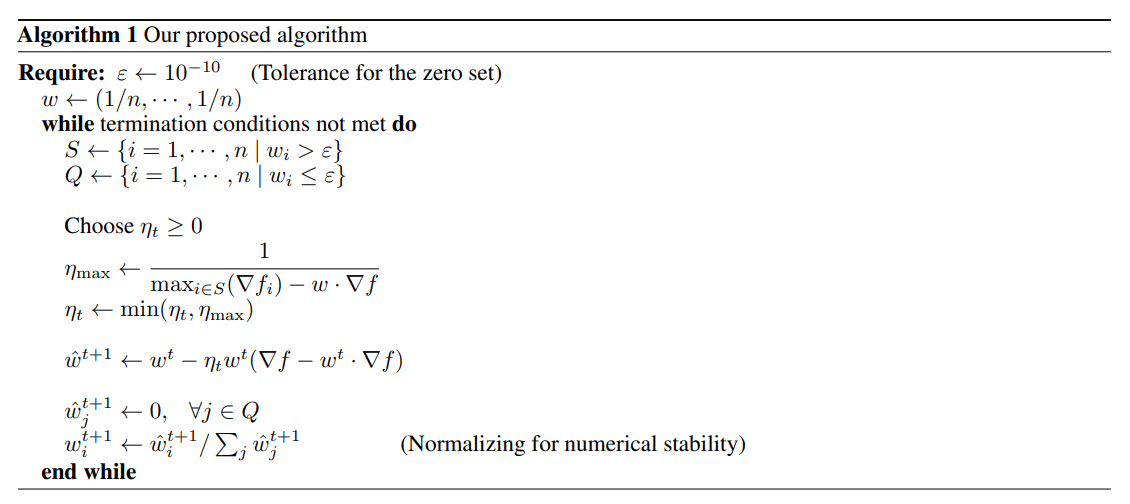
\includegraphics[width=1\linewidth]{theory/cauchy_simplex.png}
    \caption{Описание алгоритма Cauchy-Simplex}
\label{fig:cauchy_simplex}
\end{figure}

Базовый алгоритм будет состоять в следующем: на каждом шаге $t$ выбираем рычаг согласно вероятностям $\tbf{p}_t$, обновляем выборочные дисперсии и матожидания, после чего с помощью градиентного подъема находим глобальный максимум $\tbf{p}^{t+1} = (p_1^{t+1}, ..., p_n^{t+1})$ на $\Delta^n$. Далее повторяем алгоритм для $\tbf{p}_{t+1}$. Если обозначить $u$-ое значение метода градиентного подъема в ходе проведения алгоритма на шаге $t$ за $\tbf{p}_u^t$, а оптимальный вектор вероятностей на шаге $t$ за $\tbf{p}_t^*$, то тогда каждый шаг алгоритма работает за не более чем $O(k_t^{\Delta})$, где $k_t^{\Delta} = \underset{\tbf{p}^t \in \Delta^n}{\max} \min \{u: \| \tbf{p}_u^t - p_t^* \| \leq \Delta\}$ для заданной погрешности $\Delta$, так что шаг алгоритма может работать очень долго.

Кроме того, никуда не делась проблема холодного старта: аналогично итеративному алгоритму с изменением за один шаг всех вероятностей \ref{subsec:theory_iterative_change_all_probs}, после первого шага все вероятности, кроме одной $p_i^t$, могут занулиться, и далее при $Q_t(i) - S_t^2(i) > 0$ вектор вероятностей не изменится.

Изложенный выше алгоритм чем-то похож на Generalized Policy Iteration: процессом градиентного подъема можно считать policy evaluation, а нажатием рычага согласно вероятностям -- policy improvement \cite{suttonbarto_policy_iteration}. Однако здесь evaluation происходит одновременно еще и по матожиданию с дисперсией, и эти процессы друг с другом конфликтуют, что приводит к медленному или даже неверному приближению к ответу.

В заключение этого стоит заметить, что для обычной задачи о многоруком бандите как градиентный подъем, так и алгоритмы из \ref{subsec:theory_iterative} работают как обычные greedy-алгоритмы. Более того, все три алгоритма, как и стандартный greedy-алгоритм, страдают от проблемы холодного старта. Эти алгоритмы не единственны, для приближения вероятностей можно использовать метод Ньютона, метод штрафных функций, а также вместо одной или всех вероятностей пытаться за один ход изменять $k$ вероятностей, где $k = const$.

\subsection{Быстрый жадный алгоритм}
Итеративные алгоритмы обладают существенным недостатком -- каждый шаг выполняется за $O(n^2)$, что может быть слишком долго при больших размерах портфеля. Покажем алгоритм, находящий за $O(n \log n)$ распределение вероятностей, максимизирующее $Q_{t,p} - \lambda S_{t,p}^2$. Далее для удобства вместо $Q_{t,p}$ будем писать $m_p$ и вместо $S_{t,p}^2$ будем писать $\sigma_p^2$.

\subsubsection{Необходимое условие точки глобального максимума}

Пусть $i,j \in \{1, ..., n\}, \; i \neq j$. До этого мы рассматривали функцию \\
$V(p_1, ..., p_n) = m_p - \lambda \sigma_p^2$. Рассмотрим функцию
\begin{dmath}
    V(p_1, ..., p_n, \alpha) = p_1 m_1 + ... + (p_i + \alpha) m_i + ... + (p_j - \alpha) m_j + ... + p_n m_n - \lambda (p_1^2 \sigma_1^2 + ... + (p_i + \alpha)^2 \sigma_i^2 + ... + (p_j - \alpha)^2 \sigma_j^2 + ... + p_n^2 \sigma_n^2)
\end{dmath}
То есть $V(p_1, ..., p_n, \alpha) = V(p_1, ..., p_i + \alpha, ..., p_j - \alpha, ..., p_n)$. Возьмем точку $\tbf{p}^* \in \Delta^n$, в которой достигается максимум $V$ на $\Delta^n$. Предположим, что $\tbf{p}_i^* \neq 1$ и $\tbf{p}_j^* \neq 0$. Тогда $\exists \delta > 0: \: \forall \alpha: \: 0 \leq \alpha < \delta \hook \tbf{p}^*(\alpha) = (p_1^*, ..., p_i^* + \alpha, ..., p_j^* - \alpha, ..., p_n^*) \in \Delta^n$, и потому функция $V(p_1, ..., p_n, \alpha)$, определенная при $\tbf{p} \in \Delta^n, 0 \leq \alpha \leq \delta$, дифференцируема в точке $(\tbf{p}^*, 0)$ причем:
\begin{dmath}
    \frac{\partial V(p_1, ..., p_n, \alpha)}{\partial \alpha}\bigg|_{\tbf{p} = \tbf{p}^*, \, \alpha = 0} = \left( (m_i - 2\lambda p_i^* \sigma_i^2 - \alpha \lambda \sigma_i^2) + (-m_j + 2\lambda p_j^* \sigma_j^2 - \alpha \lambda \sigma_j^2) \right) \bigg|_{\alpha = 0}  = (m_i - 2 \lambda p_i^* \sigma_i^2) - (m_j - 2 \lambda p_j^* \sigma_j^2) = w_i(p_i^*) - w_j(p_j^*) 
\end{dmath}
Напомним, $w_i(p_i) = Q_t(i) - 2 \lambda p_i S_t^2(i)$ \label{eq:theory_w}. Если $\frac{\partial V}{\partial \alpha}\bigg|_{\tbf{p} = \tbf{p}^*, \, \alpha = 0} > 0$, то ввиду непрерывности $V(\alpha)$ существует $0 < \alpha < \delta: \: V(\alpha) > V(0) \land \tbf{p}(\alpha) \in \Delta^n$. Тогда максимум $V$ на $\Delta^n$ достигается не в $\tbf{p}^*$. Противоречие! $\Rightarrow \frac{\partial V}{\partial \alpha}\bigg|_{\alpha = 0} \leq 0 \Rightarrow w_i(p_i^*) \leq w_j(p_j^*)$.

\label{theory_fast_greedy_2} Пусть в точке оптимума $\tbf{p}^*$ верно, что $p_i^* \in (0,1) \land p_j^* \in (0,1)$. Тогда, подставив в предыдущий пункт сначала пару $(i,j)$, а затем $(j,i)$, получим $w_i(p_i^*) \leq w_j(p_j^*) \land w_j(p_j^*) \leq w_i(p_i^*)$, то есть $w_i(p_i^*) = w_j(p_j^*)$. Аналогично, если $p_i^* = 0 \land p_j^* \neq 0$ или $p_j^* = 1 \land p_i^* > 0$ получим $w_i(p_i^*) \leq w_j(p_j^*)$. Заметим, что если есть $i$ с $p_i = 1$, то $\forall j \neq i \hook p_j = 0$. Тогда, если $\tbf{p}^*$ -- точка оптимума на $\Delta^n$, то $\forall \, i,j: \: i \neq j \hook w_i(p_i^*) = w_j(p_j^*) = w$ и $\forall \, i,j: \: p_i^* = 0, p_j^* \neq 0 \hook w_i(p_i^*) \leq w_j(p_j^*)$, причем $\forall i \hook w_i = m_i \lrarr p_i = 0$ \label{eq:5}.

\subsubsection{Достаточное условие точки глобального максимума}
\label{subsec:theory_sufficient_condition_optimum} 

Итак, мы получили необходимое условие для точки оптимума. Является ли оно достаточным? Да, этого условия достаточно. Действительно, заметим, что $\frac{\partial V}{\partial p_i}\Bigg|_{\tbf{p}=\tbf{p}^*} = w_i(p_i^*)$. Кроме того, как мы уже показали, $\Delta^n$ выпукло и замкнуто, а $V$ нерперывно диффернцируема и вогнута на $\bb{R}^n$, и $-V$ выпукла на $\bb{R}^n$. Тогда по теореме об эквивалентном условии локального минимума на выпуклом замкнутом множестве \cite{nesterov_2_2_5} $\tbf{p}^*$ является минимумом функции $-V$ на $\Delta^n$ тогда и только тогда, когда $\forall \tbf{p} \in \Delta^n \hook \left\langle (-V)'(\tbf{p}^*), \: \tbf{p} - \tbf{p}^* \right\rangle \geq 0 \Rightarrow$ $\tbf{p}^*$ является максимумом на $\Delta^n$ тогда и только тогда, когда
\[
    \forall \tbf{p} \in \Delta^n \hook \left\langle V'(\tbf{p}^*), \: \tbf{p} - \tbf{p}^* \right\rangle \leq 0
\]
Подставим $V'$ и $\tbf{p}^*$:
\begin{dmath}
    \left\langle V'(\tbf{p}^*), \: \tbf{p} - \tbf{p}^* \right\rangle = \sum_{i=1}^n (m_i - 2\lambda p_i^* \sigma_i^2) (p_i - p_i^*) = \left( w \sum_{i: p_i^* \neq 0} p_i \right) \: + \left( \sum_{j: p_j^* = 0} m_j p_j \right) \: - \left( w \sum_{i: p_i^* \neq 0} p_i^* \right) \: - \left( \sum_{j: p_j^* = 0} m_j p_j^* \right) = w \left(1 - \sum_{j: p_j^* = 0} p_j \right) \:  + \left( \sum_{j: p_j^* = 0} m_j p_j \right) - w - 0 = \sum_{j: p_j^* = 0} (m_j - w) p_j \overset{(*)}{\leq} 0
\end{dmath}
Последнее неравенство $(*)$ верно, поскольку $\forall i,j: \: p_i = 0 \land p_j > 0 \hook m_i = w_i \leq w_j = w$.

Итак, неравенство выполнено, значит, в \ref{eq:5} описано эквивалентное условие глобального максимума на $\Delta^n$. Теперь перед описанием самого алгоритма осталось отметить пару деталей.

\subsubsection{Замечание по безрисковым рычагам}
\label{subsec:theory_notice_riskless_levers}

Пусть $m_i < m_j$. Тогда не может быть такого, что $p_i^* \neq 0 \land p_j^* = 0$. Действительно, если бы это было так, то $w_i(p_i^*) = m_i - 2 \lambda p_i^* \sigma_i^2 \leq m_i < m_j = w_j(p_j^*)$, то есть $\exists i,j: \: p_j^* = 0 \land p_i^* \neq 0 \land w_i(p_i^*) <  w_j(p_j^*)$, то есть $\tbf{p}^*$ не является точкой оптимума. Противоречие! $\Rightarrow p_i^* = 0 \lor p_j^* \neq 0$. Кроме того, если $m_i = m_j$, то $p_i^* \neq 0 \land p_j^* = 0$ возможно только в том случае, когда $\sigma_i^2 = 0$, то есть $i$-ый рычаг безрисоквый. Поэтому, если упорядочить все $m_i$ по возрастанию и сопоставить каждому $m_i$ свой $p_i^*$, то все нулевые вероятности будут находиться ``не правее'' ненулевых вероятностей, причем в какой-то точке могут находиться одновременно ненулевые и нулевые вероятности только в том случае, когда неулевым вероятностям соответствуют безрисковые рычаги.

\subsubsection{Решение на гиперплоскости $\{(p_1, ..., p_n) : \sum_{i=1}^n p_i = 1 \}$}
\label{subsec:theory_solution_outside_simplex}

Если $\forall i \sigma_i^2 > 0$ и $\exists i,\, j: \: m_i \neq m_j$, то существует метод нахождения $\tbf{p}^* = \underset{\tbf{p}}{\arg \max} (m_p - \lambda \sigma_p^2)$ на гиперплоскости $p_1 + ... + p_n = 1$ \cite{bouchaudpotters}, и для $\tbf{p}^*$ в таком случае верно, что 
\[
p_i^* = \frac{m_i}{2\lambda \sigma_i^2} + \frac{1 - \Sigma_1}{\Sigma_0} \cdot \frac{1}{2 \lambda \sigma_i^2}
\]
где
\[
\Sigma_0 = \sum_{i=1}^n \frac{1}{2 \lambda \sigma_i^2}, \; \Sigma_1 = \sum_{i=1}^n \frac{m_i}{2 \lambda \sigma_i^2}
\]
Если $m_1 = m_2 = ... = m_n = m$, то для решения $\tbf{p}^*$ верно, что $p_i^* = \frac{1}{2\sigma_i^2 \Sigma_0}$ (доказательство вкратце: фиксируем $m_p = m$, с помощью лагранжиана находим решение вида $p_i^* = \frac{\xi m + \xi'}{2\sigma_i^2}$, через ограничения находим зависимость $\xi$ и $\xi'$ от $m$, подставляем вероятности в $V$ при фиксированном $m_p = m$, получаем квадратное уравнение от $m$ с отрицательным главным коэффициентом, находим оптимальное $m$, подставляем сначала в $\xi$ и $\xi'$, а потом в $p_i^*$).\

Если же $\exists i: \: \sigma_i^2 = 0$, то есть существует безрисковый рычаг, то возьмем среди этих рычагов рычаг с наибольшим матожиданием $m_0$. Заметим, что $\exists \tbf{p}^*: \: \forall i \hook (m_i \leq m_0 \Rightarrow p_i^* = 0)$, так как можно ``перекинуть'' все такие вероятности в безрисковый рычаг, не уменьшив $V$. Если не существует рычага с матожиданием, большим $m_0$, то оптимальным решением будет всегда нажимать на рычаг с $m_0$, в противном случае существует метод нахождения $\tbf{p}^* = \underset{\tbf{p}}{\arg \max} (m_p - \lambda \sigma_p^2)$ на гиперплоскости $p_1 + ... + p_n = 1$, и 
\[p_i^* = \frac{m_i - m_0}{2 \lambda \sigma_i^2} \cdot \left(1 + m_0 \frac{\Sigma_1'}{\Sigma_2'} \right)\]
где
\[
\Sigma_k' = \sum_{i=1}^n \frac{(m_i - m_0)^k}{2 \sigma_i^2}, \: i \neq 0
\] 
То есть общее решение на гиперплоскости $p_1 + ... + p_n = 1$ существует. Также заметим, что оба алгоритма работают за $O(n)$ и что если в решении на этой гиперплоскости $\exists i: \: p_i \leq 0$, то в оптимальном решении на $\Delta^n$ существует $i$ с $p_i^* = 0$ ввиду вогнутости $V$.

\subsubsection{Описание алгоритма}

Теперь алгоритм описывается крайне просто:
\begin{enumerate}
    \item Сортируем все $m_i$ по убыванию, в случае равенства по возрастанию $\sigma_i^2$. Работает за $O(n \log n)$.
    \item С начала массива ищем безрисковый рычаг с наибольшим матожиданием. Если нашли (это первый рычаг с $\sigma_i^2 = 0$), то отбрасываем все рычаги правее найденного $\left(O(n) \right)$. 
    \item Если отбросили все рычаги, кроме безрисокового, то вероятность выбора безрискового рычага равна 1, заканчиваем работу $\left( O(1) \right)$.
    \item Иначе проходимся бинпоиском по оставшемуся массиву и находим самое левое $i=I$ такое, что в оптимальном решении с рычагами $\{1, ..., i\}$ есть $j$ с $p_j^* \leq 0$. Оптимальный вектор вероятностей находится с помощтю формул из предыдущего пункта. Каждый шаг бинпоиска работает за $O(n)$, всего шагов $O(\log n)$, поэтому бинпоиск отработает за $O(n \log n)$.
    \item Возвращаем $(p_1^*, ..., p_{I-1}^*)$ для алгоритма от рычагов $\{1, ..., I-1\}$. Отрабатывает за $O(n)$.
\end{enumerate}

\subsubsection{Доказательство работы}

Во-первых, заметим, что итоговый алгоритм работает за $O(n \log n)$. Во-вторых, уже после отбрасывания рычагов, не может быть такого, что оптимальный вектор вероятностей для рычагов $\{1,...,k\}$ выдает $\tbf{p}_k^*$, в котором $\exists i: \: p_i^* = 0$, а оптимальный вектор вероятностей для рычагов $\{1, ..., l\}, \: k < l$ выдает $\tbf{p}_l^*$, в котором $\forall i \hook p_i^* \neq 0$. Действительно, пусть для $k$ вектор вероятностей $(p_1, ..., p_{k-1}, 0)$ ($p_k = 0$, так как есть хотя бы одна нулевая вероятность и по \ref{subsec:theory_notice_riskless_levers}), а для $l$ вектор вероятностей $(q_1, ..., q_l)$, . Тогда по \ref{theory_fast_greedy_2}: $\forall i \leq k - 1 \hook m_i - 2 \lambda p_i \sigma_i^2 \geq m_k$ и $\forall i \leq k - 1 \hook m_i - 2 \lambda q_i \sigma_i^2 = m_k - 2 \lambda q_k \sigma_k^2$. Так как мы рассматриваем этап после отбрасывания рычагов и $l > k$, то $\sigma_k^2 > 0$. Тогда $m_i - 2 \lambda q_i \sigma_i^2 = m_k - 2 \lambda q_k \sigma_k^2 < m_k \leq m_i - 2 \lambda p_i \sigma_i^2 \Rightarrow p_i < q_i \Rightarrow \sum_{i=1}^{k-1} p_i = 1 < \sum_{i=1}^{k-1} q_i$. Противоречие! $\Rightarrow$ если $k < l$, то либо среди $p_i$ нет нулей, либо среди $q_i$ есть нули. Тогда, если $A_k = \{1, ..., k\}$, то индексы $A_k$ для которых в оптимальном решении нет нулевых вероятностей, образуют отрезок $\overline{1, I - 1}$, и оптимальное решение обрзовано одним из этих $I - 1$ решений.

Но заметим, что $(p_1, ..., p_k) = (p_1, ..., p_{k}, 0))$, поэтому для любого решения для $k$ рычагов с $V = V_k$ и решения для $k+1$ рычагов с $V = V_{k+1}$ верно, что $V_k \leq V_{k+1}$. Тогда решение для первых $I - 1$ рычагов -- оптимальное.

\subsection{StandardGreedy -- ускорение быстрого жадного алгоритма}

Хотя алгоритм работает за $O (n \log n)$, константа при этом значении большая, поскольку на каждом шаге бинпоиска приходится запускать алгоритм нахождения оптимального вектора вероятностей на гиперплоскости $\{(p_1, ..., p_n) : \sum_{i=1}^n p_i = 1 \}$. Оказывается, хотя с сортировкой ничего сделать нельзя, часть с бинпоиском можно заменить на другую последовательность шагов, работающую за $O(n)$. Это существенно ускорит нахождение точки оптимума. Для этого воспользуемся альтернативной формулировкой оптимума, данной в \ref{theory_fast_greedy_2} и \ref{subsec:theory_sufficient_condition_optimum}: достаточно найти такое распределение вероятностей $\tbf{p}=(p_1,...,p_n)$, что выполнено равенство \ref{eq:5}. Пусть мы отсортировали все рычаги и отбросили все, что хуже наилучшего безрискового. Посколку решение для \ref{eq:5} дает глобальный максимум на $\Delta^n$, то достаточно найти такое $t$, что $\forall i$ либо $m_i \leq t \land p_i = 0$, либо $m_i > t \land w_i = t \lrarr p_i = \frac{m_i - t}{2\lambda \sigma_i^2}$ и $\sum_{i=1}^n p_i = \sum_{i=1}^n p_i(t) = 1$. Для каждого $t$ однозначно определен набор тех $i$, для которых вероятности ненулевые, а именно такие $i$, что $m_i > t$. Кроме того, заметим, что при уменьшении $t$ сумма вероятностей увеличивается, а при $t = m_{(j)}$ (то есть $j$-ая порядковая статистика) верно, что 
\[
\sum_{i=1}^n p_i(m_{(j)}) = \sum_{i=j+1}^n \frac{m_{(i)} - m_{(j)}}{2 \lambda \sigma_{(i)}^2} = \sum_{i=j+1}^n \frac{m_{(i)}}{2 \lambda \sigma_{(i)}^2} \: - m_{(j)} \sum_{i=j+1}^n \frac{1}{2 \lambda \sigma_{(i)}^2}
\]
Если обозначить $\sum_{i=j+1}^n \frac{m_{(i)}}{2 \lambda \sigma_{(i)}^2} := \Sigma_1(j+1)$, а $\sum_{i=j+1}^n \frac{1}{2 \lambda \sigma_{(i)}^2} := \Sigma_0(j+1)$, то 
\[
\label{eq:fast}
\sum_{i=1}^n p_i(m_{(j)}) = \Sigma_1(j+1) - m_{(j)} \Sigma_0(j+1)
\]
причем $\Sigma_1(n+1) = \Sigma_0(n+1) = 0$ и $$\Sigma_1(i) = \Sigma_1(i+1) + \frac{m_{(i)}}{2\lambda \sigma_{(i)}^2}, \: \Sigma_0(i) = \Sigma_0(i+1) + \frac{1}{2\lambda \sigma_{(i)}^2}$$
Ввиду увеличения суммы вероятностей оптимальное $t$ либо лежит на полуинтервале \\ $(m_{(i)}, m_{(i+1)}]$ и $\sum_{j=1}^n p_j (m_{(i+1)}) \leq 1 < \sum_{j=1}^n p_j (m_{(i)})$, либо лежит на луче $(-\infty, m_{(1)})$ и $\sum_{j=1}^n p_j (m_{i+1}) \leq 1$. Во всех случаях мы можем вычислить $p_i$ по формулам из пункта \ref{subsec:theory_solution_outside_simplex}, учитывая только те $i$, для которых $m_{(i)} \geq t$, то есть все $m_{(i)}$ от конца интервала, где находится $t$, и до $m_{(n)}$. Итоговый алгоритм (назовем его StandardGreedy):
\begin{enumerate}
    \item Сортируем все $m_i$ по убыванию, в случае равенства по возрастанию $\sigma_i^2$. Работает за $O(n \log n)$.
    \item С начала массива ищем безрисковый рычаг с наибольшим матожиданием. Если нашли (это первый рычаг с $\sigma_i^2 = 0$), то отбрасываем все рычаги правее найденного $\left(O(n) \right)$. 
    \item Если отбросили все рычаги, кроме безрискового, то вероятность выбора безрискового рычага равна 1, заканчиваем работу $\left( O(1) \right)$.
    \item Иначе считаем $\Sigma_1(n+1) = \Sigma_0(n+1) = 0$, проходимся слева направо по $m_{(i)}$, пересчитывая за $O(1)$ $\Sigma_1(i+1)$ и $\Sigma_0(i+1)$, вычисляя за $O(1)$ по формуле \ref{eq:fast} сумму вероятностей. Находим первое такое $i$, что $\sum_{i=1}^n p_i(m_{(i+1)}) \leq 1$ и $\sum_{i=1}^n p_i(m_{(i+1)}) > 1$ $\left( O(n) \right)$.
    \item Если такое $i$ нашлось, то $p_j$ для $j \geq i + 1$ вычисляются по формулам из пункта \ref{subsec:theory_solution_outside_simplex} а для $j \leq i \hook p_j = 0$. Если же не нашлось, то у всех рычагов ненулевые вероятности, и, аналогично, по формулам из пункта \ref{subsec:theory_solution_outside_simplex} вычисляются все $p_i$ $\left( O(n) \right)$.
\end{enumerate}

Псевдокод алгоритма StandardGreedy дан ниже (\ref{lst:theory_asset_def}, \ref{lst:theory_standardgreedy_def}, \ref{lst:theory_calc_opt_probs_on_subsimplex_def}):

\begin{algorithm}
\caption{Asset Struct Definition}
\label{lst:theory_asset_def}
\begin{algorithmic}[1]
\STATE \textbf{Struct} Asset
\STATE \quad \textbf{Field} mean: \textbf{float}
\STATE \quad \textbf{Field} var: \textbf{float}
\STATE \quad \textbf{Field} idx: \textbf{int}
\end{algorithmic}
\end{algorithm}

\begin{algorithm}
\caption{StandardGreedy algorithm}
\label{lst:theory_standardgreedy_def}
\begin{algorithmic}[1]
\STATE \textbf{Input:} means, variances, $\lambda$
\STATE Zip means, vars and indexes in these arrays to $A$[Asset] // array of ``assets''
\STATE Sort $A$ by mean in descending order and var in ascending order

\STATE Find first index highest\_safe\_lever\_idx in $A$ with var = 0 (if absent then highest\_safe\_lever\_idx $\gets len(A)$)

\IF{highest\_safe\_lever\_idx == 0}
    \STATE $p_{opt} \gets [0] \cdot len(A)$
    \STATE $p_{opt}[A[0].idx] \gets 1$
    \STATE \textbf{return} $p_{opt}$
\ENDIF

\STATE safe\_lever\_exists $\gets$ (highest\_safe\_lever\_idx $ \neq len(A)$)
\STATE $\Sigma_0 \gets 0$,  $\Sigma_1 \gets 0$
\FOR{i from 1 to highest\_safe\_lever\_idx + 1 if safe\_lever\_exists else $len(A)$}
    \STATE $\Sigma_0 \gets \Sigma_0 + \frac{1}{2 \lambda \cdot A[i - 1].var}$
    \STATE $\Sigma_1 \gets \Sigma_1 + \frac{A[i - 1].mean}{2 \lambda \cdot A[i - 1].var}$
    \IF{$\Sigma_1 - \Sigma_0 \cdot A[i].mean \geq 1$}
        \STATE \textbf{return} calc\_$p_{opt}$\_on\_subsimplex($A, i, False, \lambda$)
    \ENDIF
\ENDFOR
\STATE \textbf{return} calc\_$p_{opt}$\_on\_subsimplex($A, \text{highest\_safe\_lever\_idx}, \text{safe\_lever\_exists}, \lambda$)
\end{algorithmic}
\end{algorithm}

\begin{algorithm}
\caption{calc\_$p_{opt}$\_on\_subsimplex Function}
\label{lst:theory_calc_opt_probs_on_subsimplex_def}
\begin{algorithmic}[1]
\STATE \textbf{Input:} $A$, end\_range, safe\_lever\_exists, $\lambda$
\STATE $p_{opt} \gets [0] \cdot len(A)$
\STATE $\Sigma_0 \gets 0$,  $\Sigma_1 \gets 0$
\IF{not safe\_lever\_exists}
    \FOR{each $i$ from 0 to end\_range - 1}
        \STATE $\Sigma_0 \gets \Sigma_0 + \frac{1}{2 \lambda \cdot A[i].var}$
        \STATE $\Sigma_1 \gets \Sigma_1 + \frac{A[i].mean}{2 \lambda \cdot A[i].var}$
    \ENDFOR
    \FOR{each $i$ from 0 to end\_range - 1}
        \STATE $p_{opt}[A[i].idx] \gets \frac{A[i].mean}{2 \lambda \cdot A[i].var} + \frac{1 - \Sigma_1}{\Sigma_0 \cdot 2 \lambda \cdot A[i].var}$
    \ENDFOR
\ELSE
    \STATE $p_{sum} \gets 0$
    \FOR{each $i$ from 0 to end\_range - 1}
        \STATE $p_{opt}[A[i].idx] \gets \frac{A[i].mean - A[\text{end\_range}].mean}{2 \lambda \cdot A[i].var}$
        \STATE $p_{sum} \gets p_{sum} + p_{opt}[A[i].idx]$
    \ENDFOR
    \STATE $p_{opt}[A[\text{end\_range}].idx] \gets 1 - p_{sum}$
\ENDIF
\STATE \textbf{return} $p_{opt}$
\end{algorithmic}
\end{algorithm}

Алгоритм работает за $O(n \log n)$, но при этом быстрее, чем прошлый, так как часть после сортировки работает за $O(n)$, а не за $O(n \log n)$. Интересно заметить, что мы ищем первое такое $t$, что $\sum_{j=i+1}^n \frac{m_{(j)} - t}{2\lambda \sigma_{(j)}^2} = 1 \lrarr t = \frac{\Sigma_1(i+1) - 1}{\Sigma_0(i+1)}$, а это похоже на формулы из статьи ``Projection onto a simplex'' \cite{simplex_projection}.

\subsection{Замена максимизации на ``выравнивание''}
\label{subsec:theory_alignment}

Вообще стоит указать, что нам не так важна максимизация $V = m_p - \lambda \sigma_p^2$. Скорее, нам важна величина $\frac{\partial V}{\partial p_i}\Bigg|_{p_i = p_i^*} = w_i(p_i^*)$. Мы хотим найти такое распределение вероятностей, что 
\[
    \forall i,j \hook (p_i^* = 0 \land p_j^* \neq 0 \Rightarrow w_i(p_i^*) \leq w_j(p_j^*))
\]
и что 
\[
    \forall i,j \hook (p_i^* \neq 0 \land p_j^* \neq 0 \Rightarrow w_i(p_i^*) = w_j(p_j^*))
\]
Более того, в оригинальной задаче о многоруких бандитах требуется максимизировать $V = m_p$, что равносильно нахождению такого вектора вероятностей $(p_1^*, ..., p_n^*)$, что 
\[
    \forall i,j \hook \left(p_i^* = 0 \land p_j^* \neq 0 \Rightarrow \frac{\partial V}{\partial p_i}\Bigg|_{p_i = p_i^*} = m_i \leq m_j = \frac{\partial V}{\partial p_j}\Bigg|_{p_j = p_j^*} \right)
\]
и что 
\[
    \forall i,j \hook \left(p_i^* \neq 0 \land p_j^* \neq 0 \Rightarrow \frac{\partial V}{\partial p_i}\Bigg|_{p_i = p_i^*} = m_i = m_j = \frac{\partial V}{\partial p_j}\Bigg|_{p_j = p_j^*} \right)
\]
(см. \ref{subsec:theory_sufficient_condition_optimum}). Этим соображением мы воспользуемся при адаптировании метода Gradient bandits.

\section{Некоторые способы избавления от проблемы холодного старта}

Все вышеперечисленные алгоритмы страдают от пролемы холодного старта: приближения матожидания и дисперсии в начале обладают большим разбросом, из-за чего вероятности выбора некоторых рычагов могут обнулиться, и эти рычаги больше не будут выбираться, хотя эти рычаги могут иметь большую вероятность в оптимальном векторе $\tbf{p}$. Все дальнейшие стратегии стараются избавиться от этой проблемы. В этом небольшом параграфе даются специфичные для предложенных выше алгоритмов способы борьбы с проблемой холодного старта.

Для градиентного подъема можно использовать две техники:
\begin{enumerate}
    \item На каждом шаге делать лишь $k$ итераций градиентного подъема. Как крайний вариант этой техники, на каждом шаге можно производить всего одну итерацию, в таком случае стратегия становится похожа на value iteration \cite{suttonbarto_value_iteration}.
    \item После нахождения оптимума $\tbf{p}^*$ смещаться на случайный вектор, уменьшающийся по модулю со временем.
\end{enumerate}

Для итеративного метода, изменяющего каждый ход только две вероятности, можно ограничивать максимальный вектор, на который можно смещаться, взяв $\Delta p_{final} = \min (\frac{p_i}{2}, \Delta p)$. Эта техника легко адаптируется для итеративного метода с изменением всех вероятностей.

Наконец, как метод, заменяющий на начальном этапе другие стратегии и алгоритмы, можно прожать на каждый рычаг определенное число раз, чтобы иметь приближения $m_i$ и $\sigma_i^2$. В крайнем случае можно нажать по разу или по 2 раза, чтобы посчитать дисперсию.

\section{$\epsilon$-greedy стратегии}

В классической задаче о многоруких бандитах $\epsilon$-greedy стратегии -- это стратегии, действие на $t$-ом шаге в которых вычисляется по формуле:
\[
A_t = \begin{cases}
           \underset{a}{\arg \max} \; Q_t(a), & \text{with probability} \; 1 - \epsilon, \\
           \text{a random action}, & \text{with probability} \; \epsilon.
       \end{cases}
\]
Поскольку в измененной задаче о мноруких бандитах выбор каждого рычага вероятностный, в адаптированной версии $\epsilon$-greedy будем выбирать рычаг согласно вероятностному вектору $\tbf{p}_t$, где
\[
\tbf{p}_t = 
    \begin{cases}
           \text{StandardGreedy}(Q_t, S_t^2, \lambda) & \text{with probability} \; 1 - \epsilon, \\
           \left( \frac{1}{n}, ..., \frac{1}{n} \right), & \text{with probability} \; \epsilon.
    \end{cases}
\]

Заметим, что в такой формулировке $\epsilon$ не меняется со временем, хотя при увеличении числа шагов приближения $m_i$ и $\sigma_i^2$ становятся точнее. Поэтому можно ввести стратегии с адаптивным $\epsilon$. \href{https://en.wikipedia.org/wiki/Multi-armed_bandit}{Например}:
\begin{enumerate}
    \item На $t$-ом шаге $\epsilon_t = \min(1, \frac{\epsilon_0}{t})$ \cite{srank}. Назовем стратегию Adaptive-$\epsilon$
    \item VDBE: см. рис. \ref{fig:VDBE_epsilon}:
    \begin{figure}
        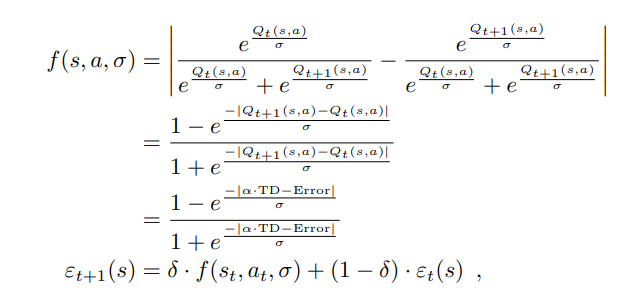
\includegraphics[width=0.8\linewidth]{theory/VDBE_epsilon.png}
        \caption{\label{fig:VDBE_epsilon} Алгоритм VDBE. На $s$ можно не обращать внимания, $a$ -- выбранное на $t$-ом шаге действие, $\sigma$ -- температура: чем выше, тем ближе распределение к равномерному, чем меньше, тем ближе к жадному \cite{tolic_VDBE}}
    \end{figure}
    Формулы из VDBE, который предназначался для модели марковского процесса принятия решений (МППР), адаптируются следующим образом:
    \[
    f(A_t, \tau) = \left| \frac{e^{\frac{Q_t(A_t)}{\tau}} - e^{\frac{Q_{t + 1}(A_t)}{\tau}}}{e^{\frac{Q_t(A_t)}{\tau}} + e^{\frac{Q_{t + 1}(A_t)}{\tau}}} \right|,
    \]
    \[
    \epsilon_{t+1} = \delta \cdot f(A_t, \tau) + (1 - \delta) \cdot \epsilon_t
    \]
\end{enumerate}
Также в дальнейшем мы обсудим коррекцию дисперсии, однако это будет в секции экспериментов.

\section{Позитивная инициализация}

В обычной задаче о многоруких бандитах стратегии с позитивной инициализацией -- это стратегии, для которых изначально $\forall a \; Q_t(a) = d, \; d > 0$. Такой прием помогает на первых шагах прожать каждый из рычагов хотя бы по одному разу, что увеличивает точность приближений. Часто обновление $Q_t(A_t)$ происходит с константынм шагом (хотя это и не принципиально), то есть если на шаге $t$ было выбрано действие $a$, то для всех остальных действий $b$ значение $Q_t(b)$ не меняется, а для действия $a$ $Q_t(a) = Q_t(a) + \alpha (R_t - Q_t(a)), \; \alpha = const$. $\alpha$ называется step-size.

В измененной задаче можно так же инициализировать начальные значения всех рычагов большим положительным числом, как и в обычной позитивной инициализации. Обновление $Q_t(a)$ происходит с константынм шагом (step-size) в соответствии с материалом \href{https://matteosantama.github.io/ewm/}{на этой странице}. В соответствии с тем же материалом меняется $S_t^2(a)$.

\section{UCB}
В классической задаче выбор в стратегии UCB строился по формуле
\[
A_t = \underset{a}{\arg \max} \; \left[ Q_t(a) + c \sqrt{\frac{\ln \; t}{N_t(a)}} \right], \; c > 0
\]
То есть вместо $Q_t(a)$ в формулу для жадной стратегии подставляется верхняя граница доверительного интервала для $Q_t(a)$. Так как в начале $N_t(a) = 0$ для любого рычага, то часто вместо $N_t(a)$ в знаменателе подставляют $N_t(a) + \epsilon$, где $\epsilon >0$ -- очень маленькое число. Идея использования значения $\sqrt{\frac{\ln \; t}{N_t(a)}}$ в качестве ``добавки'' к $Q_t(a)$ строится на неравенстве Хаффдинга \cite{intro_bandits_ucb}:
\[
\bb{P}\left( |Q_t(a) - m_a| \geq \sqrt{\frac{\alpha \beta \ln t}{N_t(a)}} \right) \leq 2 t^{-2 \alpha}
\]
где для гауссовских случайных величин $\beta = 4 \sigma^2$. Уже для распределений Стьюдента неравенство не выполняется, что может создать проблемы даже для обычной задачи о многоруких бандитах. За неимением лучшего в обычной задаче будем использовать $\sqrt{\frac{\ln \; t}{N_t(a)}}$ для верхней границы $Q_t(a)$ для всех распределений.

Для измененной задачи о многоруких бандитах неравенство Хаффдинга все еще остается верным для матожидания. В случае с дисперсией аналог неравенства Хаффдинга не выполняется даже для нормального распределения, поскольку ``хвосты'' выборочной дисперсии слишком тяжелые: $\frac{S_t^2(a)}{\sigma_a^2} \sim \chi_{t-1}^2$, в то время как $Q_t(a) - m_a \sim \mathcal{N}(0, \frac{\sigma_a^2}{n})$. Для распределений Стьюдента дело обстоит еще хуже: для $t_{\nu}$ с $\nu < 4$ у распределения $S_t^2$ не существует дисперсии. В связи с этим возьмем самую простую версию UCB с модификацией исключительно матожидания:
\[
\tbf{p}_t = \text{StandardGreedy}\left(Q_t + c \sqrt{\frac{\ln t}{N_t}}, S_t^2, \lambda \right)
\]

\section{Gradient bandits}

В классической задаче в стратегии gradient bandits для каждого действия $a$ вводится значение $H_t(a)$ \cite{suttonbarto_gradient_bandits}. На первом шаге $\forall a \hook H_1(a) = 0$. На $t$-ом шаге выбор происходит среди действий соответственно вероятностям $\bb{P}\{A_t = a\} = \frac{e^{H_t(a)}}{\sum_{i=1}^{k} e^{H_t(i)}} := \pi_t(a)$. После выбора действия $A_t$ и получения награды $R_t$ обновления $H_t$ происходят по формулам:
\[
\begin{aligned}
  & H_{t+1}(A_t) = H_t(A_t) + \alpha (R_t - \bar{R_t}) (1 - \pi_t(A_t)), \; \text{and} \\ 
  & H_{t+1}(a) = H_t(a) - \alpha (R_t - \bar{R_t})\pi_t(a), \; a \neq A_t.
\end{aligned}
\]
где $\bar{R_t} = \frac{\sum_{i=1}^{t-1} R_i}{t - 1}$ -- baseline ($\bar{R_1} = 0$). Если полученная награда при нажатии на рычаг $R_t$ больше $\bar{R_t}$, то нажатие на рычаг увеличивает средний выигрыш, и предпочтение рычага $A_t$ увеличивается, а остальных рычагов -- уменьшается. Если же $R_t < \bar{R_t}$, то движение происходит в обратную сторону. Заметим, что $\bar{R_t}$ -- это взвешенное среднее всех $Q_t(a)$:
\[
\bar{R_t} = \sum_{i=1}^n \frac{N_t(a)}{t - 1} Q_t(a)
\]

Выведем похожую формулу для измененной задачи, проведя аналогичные вычисления, что и в книге ``Reinforcement Learning: An Inrtroduction'' \cite{suttonbarto_gradient_bandits}. Воспользуемся методом градиентного подъема в пространстве $H_t$ предпочтений выбора каждого рычага. Каждый ход предпочтения будут меняться пропорционально изменению $V(Q_t, S_t^2, \lambda)$:
\[
    H_{t+1}(a) = H_t(a) + \alpha \frac{\partial \bb{E}(Q_{t,\pi} - \lambda S_{t,\pi}^2)}{\partial H_t(a)}
\]
Для удобства опять заменим $Q_{t}(a) = m_a, \: S_t^2(a) = \sigma_a^2$. Распишем градиент подробнее:
\begin{dmath}
    \frac{\partial \bb{E}(m_{\pi} - \lambda \sigma_{\pi}^2)}{\partial H_t(a)} = \sum_{x} \left( m_x - 2 \lambda \pi_t(x) \sigma_x^2 \right) \frac{\partial \pi_t(x)}{\partial H_t(a)} = \bb{E} \left( \frac{m_{A_t}}{\pi_t(A_t)} - 2 \lambda \sigma_{A_t}^2 - B_t \right) \frac{\partial \pi_t(A_t)}{\partial H_t(a)} = \bb{E} \left( m_{A_t} - 2 \lambda \pi_t(A_t) \sigma_{A_t}^2 - B_t \right) \left( \bb{I}_{a=A_t} - \pi_t(a) \right) = \bb{E} \left( Q_{t+1}(A_t)  - 2 \lambda \pi_t(A_t) S_{t+1}^2 (A_t) - B_t \right) \left( \bb{I}_{a=A_t} - \pi_t(a) \right)
\end{dmath}
Последний переход верен, поскольку $\bb{E} [Q_{t+1}(a) | a=A_t] = \bb{E} [R_t | A_t] = m_{A_t}$ и $\bb{E} [S_t^2(a) | a=A_t] = \sigma_{A_t}^2$. В отличие от классической задачи, мы взяли $Q_{t+1}(a)$ вместо $R_t$ в формуле для большей стабильности.

Осталось выбрать baseline. Возьмем средневзвешенное всех $w_t(a)$ (\ref{eq:theory_w}):
\[
B_t := \bar{w_t} = \sum_{a=1}^n \frac{N_t(a)}{t-1} \left( Q_t(a) - 2 \lambda \pi_t(a) S_t^2(a) \right)
\]
При 
Заметим, что baseline работает, в первую очередь, не для максимизации $V$, а для ``выравнивания'' $w_t$ (\ref{subsec:theory_alignment}): если $ Q_{t+1}(A_t)  - 2 \lambda \pi_t(A_t) S_{t+1}^2 (A_t) > B_t$, то увеличение предпочтения для рычага $A_t$ приведет к увеличению $V$, в результате вероятность выбора рычага $A_t$ увеличится, $w_t(A_t)$ уменьшится, что заставит $w_t(A_t)$ выровняться относительно baseline при следующем выборе рычага $A_t$. Аналогично, если $< B_t$. Таким образом, градиентные бандиты ``отбирают'' рычаги, приводящие к выравниванию baseline с $w_t(A_t)$. 
Итоговая формула:
\[
\begin{aligned}
  & H_{t+1}(A_t) = H_t(A_t) + \alpha \left( w_t(A_t) - \sum_{a=1}^n \frac{N_t(a)}{t-1} w_t(A_t) \right) (1 - \pi_t(A_t)), \; \text{and} \\ 
  & H_{t+1}(a) = H_t(a) - \alpha  \left( w_t(A_t) - \sum_{a=1}^n \frac{N_t(a)}{t-1} w_t(A_t) \right) \pi_t(a), \; a \neq A_t.
\end{aligned}
\]
Храня вектор всех $w_t(a)$ (каждый шаг надо менять всего одну ячейку $w$), а также храня $B_t$, можно пересчитывать $B_t$ за $O(1)$ по формуле:
\begin{dmath}
    B_{t+1} = \frac{(t-1)B_t - N_t(A_t) w_t(A_t) + (N_t(A_t) + 1) w_{t+1}(A_t)}{t}
            = B_t + \frac{1}{t} \left[ N_t(A_t) \left( w_{t+1}(A_t) - w_t(A_t) \right) + w_{t+1}(A_t) - B_t \right]
\end{dmath}
Тогда и пересчет каждого $H_t(a)$ можно производить за $O(1)$ (хотя без распараллеливания суммарный подсчет $H_t$ и $\pi_t$ будет происходить за $O(n)$).

\section{Альтернативные стратегии}

\subsection{Сэмплирование Томпсона}

Если нам известно, из какого семейства распределений взяты распределения для рычагов (например, из гауссовского распределения), то в некоторых случаях можно найти сопряженное семейство распределений. Тогда для обычной задачи о многоруких бандитах можно использовать алгоритм, известный как сэмплирование Томпсона \cite{intro_bandits}: можно считать, что параметры исходного семейства распределений были взяты, исходя из сопряженного семейства распределений. В таком случае, хоть нам и неизвестны исходные параметры, но мы можем оценить их апостериорную вероятность. Исходный алгоритм выглядит так:
\begin{enumerate}
    \item Для каждого рычага сэмплируются матожидания в соответствии своим апостериорным вероятностям
    \item Выбирается рычаг с максимальным сэмплированным матожиданием
    \item Для выбранного рычага выдается награда и обновляются параметры для распределения из сопряженного семейства распределений, соответствующего этому рычагу. Тем самым изменяется представление о том, чему равно матожидание для выбранного рычага.
    \item Возврат к шагу 1.
\end{enumerate}
Сэмплирование Томпсона обладает весомым достоинством -- оно очень быстро находит рычаг с наибольшим матожиданием. А именно: матожидание сожаления $\bb{E} \: \overline{\text{Regret}_T} = O\left(\sqrt{n \frac{\log T}{T}} \right)$, где
\[
\overline{\text{Regret}_t} = \left[ \underset{\tbf{p} \in \Delta^n}{\max} \left( \frac{\sum_{k=1}^t m_{p_k} - \lambda \sigma_{p_k}^2}{t} \right) \right] - (m_{p_t} - \lambda \sigma_{p_t}^2)
\]
Это значительный результат, поскольку, например, для любой стратегии с неадаптивным (то есть не зависящим от истории наград) исследованием при фиксированных $T, n$ существуют распределения на рычагах, при которых  $\bb{E} \: \overline{\text{Regret}_T} \geq \Omega \left(n^{1/3} \, T^{-1/3} \right)$ \cite{intro_bandits_slow_convergence}.

Сэмплирование Томпсона можно обобщить для случаев, когда выбор рычага не детерминирован. Рассмотрим такую модификацию для нашей задачи:
\begin{enumerate}
    \item Для каждого рычага сэмплируются матожидания и дисперсии в соответствии со своими апостериорными вероятностями.
    \item С помощью StandardGreedy для выбранных матожиданий и дисперсий находится $\tbf{p}^* = \underset{\tbf{p} \in \Delta^n}{\arg \max} (m_{\tbf{p}} - \lambda \sigma_{\tbf{p}}^2)$
    \item Выбирается рычаг в соответствии с $\tbf{p}^*$.
    \item Для выбранного рычага выдается награда и обновляются параметры для распределения из сопряженного семейства распределений, соответствующего этому рычагу. Тем самым изменяется представление о том, чему равны матожидание и дсиперсия для выбранного рычага.
    \item Возврат к шагу 1.
\end{enumerate}

Предполагается, что алгоритм будет отлично работать для рычагов, распределения которых гауссовские. Однако для распределения Стьюдента возникают серьезные трудности, поскольку даже при известном числе степеней свободы для семейства распределений Стьюдента не существует сопряженного распределения \cite{conjugate_priors}. Однако есть способ с помощью суммы других распределений приблизить сопряженное распределение \cite{approx_of_conjugate_prior}. Изучение результатов задачи о многоруких бандитах при применении сэмплирования Томпсона с приближением сопряженным распределения может стать интересной темой дальнейшего исследования.

\subsection{Альтернативный подход к изменению вероятностей}

Для аппроксимации оптимума в измененной задаче можно рассмотреть совсем другой подход: На $t$-ом шаге будем считать, что $p_t^i = \frac{N_t(i)}{t-1}$, таким образом, вероятности формируются в зависимости от того, насколько часто выбирали рычаг. Далее можно посчитать $w_i = Q_t(i) - 2 \lambda p_i S_t^2(i)$ для каждого $i$ и взять рычаг для нажатия, исходя из максимума $w_i$. По сути, нам необходимо найти такое распределение вероятностей, что для ненулевых вероятностей $w_i = w_j$, а все остальные $w_k$ не больше. Здесь возникает та же проблема холодного старта, но дополнительно на дальних шагах сложно изменить вероятности. Возможно, стоит отдавать большее ``предпочтение'' последним выборам рычагов (их вес больше веса других вероятностей). Или считать нажатия рычагов только в определенном окне (тогда снизится точность).

Этот подход можно применить для UCB: аналогично классическому UCB, \\
$A_t = \underset{a}{\arg \max} \left( Q_t(a) - 2 \lambda p_a S_t^2(a) + c \sqrt{\frac{\ln t}{N_t(a)}} \right)$, где $p_a = \frac{N_t(a)}{t-1}$.